\subsection{Value chain}


Porter's value chain model beskriver et firma ud fra de aktiviteter der skal udføres for at tilføje værdi til de "rå" materialer.
Eftersom modellen er konstrueret med konventionelle fremstillingsvirksomheder i tankerne kan det ikke direkte overføres til softwarevirksomheder.
Softwarevirksomheder inkøber sjældent rå materialer i traditionel forstand, men ideerne gælder stadig på et konceptuelt niveau.

Følgendende beskrivelse er baseret på \citet[p.~12]{rose2012software}.

Aktiviterer inddeles i to kategorier, de primære og support aktiviteter.
De primære aktiviteter beskriver hvordan virksomheden omdanner rå materialer til det færdige produkt på hylden ved at tilføje værdi.
Modellen er illustreret på  \cref{valuechain}.

\begin{figure}
	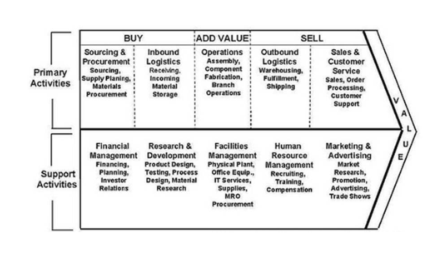
\includegraphics[width=\textwidth]{valuechain.png}
	\caption{Porters valuechain model}
	\label{valuechain}
\end{figure}

\paragraph{Application}
We have used 

\subsubsection*{Primary activities}
BUY:
\begin{itemize}
\item NFC kort
\item Fysisk login med NFC kort hos firma - her opdateres passwords på kortet
\end{itemize}
ADD VALUE:
\begin{itemize}
\item Sikkerhedsprotokol mellem fysisk login portal og server
\item Sikkerhedsprotokol mellem klient og NFC kort
\item Sikkerhedsprotokol mellem fysisk login portal og NFC kort
\item Software til password server
\end{itemize}
SELL:
\begin{itemize}
\item Sælg bedste produkt i verden
\item Tjen en masse penge på support
\end{itemize}

\subsubsection*{Support activities}
SELL
\begin{itemize}
\item Marketing
\item Hyre - sikkerhedsekspert, hardwaredesigner
\end{itemize}